\newcommand{\anonsection}[1]{\section*{#1}\addcontentsline{toc}{section}{#1}}
\newcommand{\anonsubsection}[1]{\subsection*{#1}\addcontentsline{toc}{subsection}{#1}}
\newcommand{\anonsubsubsection}[1]{\subsubsection*{#1}\addcontentsline{toc}{subsubsection}{#1}}
\documentclass[10pt]{article}
\usepackage{a4wide}
\usepackage[utf8]{inputenc}
\usepackage[russian]{babel}
\usepackage{graphicx}
\usepackage{amsmath}
\usepackage{amsfonts}
\usepackage{caption}
\usepackage{subfig}
\usepackage[left=3cm,right=3cm, top=3cm,bottom=3cm,bindingoffset=0cm]{geometry}
\usepackage{hyperref}

\newtheorem{theorem}{Теорема}
\newtheorem{definition}{Определение}
\newtheorem{notion}{Замечание}

\begin{document}

\thispagestyle{empty}

\begin{center}
\ \vspace{-3cm}


\includegraphics[width=0.5\textwidth]{msu.png}\\
{\scshape Московский государственный университет имени М.~В.~Ломоносова}\\
Факультет вычислительной математики и кибернетики\\
Кафедра системного анализа

\vfill

{\LARGE Отчет о практическом задании по курсу ``Оптимальное управление'' }

\vspace{1cm}

{\Huge\bfseries <<Задача управления тележкой>>}
\end{center}

\vspace{1cm}

\begin{flushright}
  \large
  \textit{Студент 315 группы}\\
  Е.\,В.~Гуров

  \vspace{5mm}

  \textit{Руководитель практикума}\\
  к.ф.-м.н., доцент П.\,А.~Точилин
\end{flushright}

\vfill

\begin{center}
Москва, 2021
\end{center}
\newpage

\tableofcontents
\newpage

\anonsection{Постановка задачи}
Движение материальной точки на прямой описывается обыкновенным дифференциальным уравнением:
\begin{equation} \label{dif_equation}
	 \ddot{x} = u_1 - \dot{x}(1 + u_2) \ , \ t \in [0,T], 
\end{equation}
где \( x \in \mathbb{R} \ , \ u = (u_1, u_2)^{\text{T}} \in \mathbb{R}^2 \). На возможные значения управляющих парметров \( u_1, u_2 \) наложены следующие ограничения:
\begin{enumerate}
	\item либо \( u_1 \ge u_{min} \ge 0 \ , \ u_2 \in [-k,k] \ , \ k > 0 \),
	\item либо \( u_1 \in \mathbb{R} \ , \ u_2 \in [-k,k] \ , \ k > 0\).
\end{enumerate}
Задан начальный момент времени \( t_0 = 0 \) и начальная позиция \( x(0) = 0 \ , \ |\dot{x}(0)| \le \varepsilon \). Необходимо за счет выбора программного управления \( u \)  перевести материальную точку из заданной начальной позиции в такую позицию в момене времени \( T \), в которой \( x(T) = L \ge 0 \ , \ |\dot{x}(T)| \le \varepsilon \). На множестве всех реализаций программных управлений, переводящих систему в указанное состояние, необходимо решить задачу оптимизации:
\[ J = \int\limits_0^T u_1^2(t)dt \to \min\limits_{u(\cdot)} \]
\begin{itemize}
\item Необходимо написать в среде MatLab программу с пользовательским интерфейсом, которая по заданным параметрам \( T, k, L, \varepsilon, u_{min} \) определяет, разрешима ли задача оптимального управления(при одном из указанных двух ограничений на управления). Если задача резрешима, то программа должна построить графики компонент оптимального управления, компонент оптимальной траектории, сопряженных переменных. Кроме того, программа должна определить количество переключений найденного оптимального управления, а также моменты переключений.
\item В соответствующем заданию отчете необходимо привести все теоретические выкладки, сделанные в ходе решения задачи оптимального управления, привести примеры построенных оптимальных управлений и траекторий(с иллюстрациями). Все вспомогатльные утверждения(за исключением принципа максимума Понтрягина), указанные в отчете должны быть доказаны. В отчете должны быть приведены примеры оптимальных траекторий для всех возможных качественно различных ``режимов''.
\end{itemize}

\noindent \textbf{Замечание.} Алгоритм построения оптимальной траектории не должен содержать перебор по параметрам, значения которых не ограничены, а также по более чем двум скалярным параметрам.
\newpage
\anonsection{Теоретическая часть}
\anonsubsection{Интерпретация условия}
Для начала решения задачи следует разобраться с интерпретацией условия и входящих в него параметров:
\begin{enumerate}
	\item \( x \) --- координата тележки на прямой. \( \ddot{x} \) и \( \dot{x} \) --- ускорение и скорость тележки соотвественно.
	\item \( u_1 \) --- варьируемое ускорение, придаваемое тележкой некоторой сторонней силой. В случае первых ограничений на управление ``толкать'' возможно только в положительном напрвлении координатной оси \( x \), придавая дополнительное ускорение не меньшее некоторого \( u_{min} \). Во втором случае ``толкать'' возможно в любом напрвлении, придавая любое дополнительное ускорение тележке.
	\item \( u_2 \) --- варьируемый параметр, играющий роль коэффициента трения о воздух. В данном случае возможно некоторым образом управлять плотностью или составом среды, в которой движется тележка(в некоторых задаваемых границах от \( [-k; k] \ , \ k > 0 \)). Отрицательный коэффициент трения возможен.
	\item Задача состоит в том, чтобы доставить тележку во время \( T \) на расстояние \( L \) в положительном напрвлении по оси координат(\( L > 0\)), затратив меньше всего ``усилий'' сторонней силой.
\end{enumerate}
\anonsubsection{Принцип максимума Понтрягина}
Начнем анализ задачи с формулировки принципа максимума Понтрягина. Для этого сведем уравнение (\ref{dif_equation}) к системе дифференциальных уравнений. Положим \( x_1 = x \ , \ x_2 = \dot{x} \). Получим систему:
\begin{equation} \label{dif_system}
	\begin{cases}
		\dot{x}_1 = x_2, 
		\\
		\dot{x}_2 = u_1 - x_2(1 + u_2).
	\end{cases}
\end{equation}
Введем обозначения:
\[ x = \begin{pmatrix} x_1 \\ x_2 \end{pmatrix} \ , \ \psi = \begin{pmatrix} \psi_1 \\ \psi_2 \end{pmatrix} \ , \  u = \begin{pmatrix} u_1 \\ u_2 \end{pmatrix} \ , \ \overline{x} = \begin{pmatrix} x_0 \\ x_1 \\ x_2 \end{pmatrix} \ , \ \overline{\psi} = \begin{pmatrix} \psi_0 \\ \psi_1 \\ \psi_2 \end{pmatrix} \ , \ \overline{f}(x,u) = \begin{pmatrix} u_1^2 \\ x_2 \\ u_1 - x_2(1 + u_2) \end{pmatrix} \]
\[ \mathcal{X}_0 = \{x = (x_1,x_2)^{\text{T}} | \ x_1 = 0, |x_2| < \varepsilon \}, \]
\[ \mathcal{X}_1 = \{x = (x_1,x_2)^{\text{T}} | \ x_1 = L, |x_2| < \varepsilon \}. \]
С помощью них можно перейти к эквивалентной форме задачи:
\[ \begin{cases} \dot{\overline{x}} = \overline{f}(x, u), \\ x_0(T) \to \inf\limits_{u \in \mathcal{P}} \end{cases} \]
Выпишем функцию Гамильтона-Понтрягина и ее точную верхнюю грань по \( u \):
\[ \mathcal{H}(x, u, \overline{\psi}) = \langle \overline{\psi}, \overline{f}(x,u) \rangle = \psi_0u_1^2 + \psi_1x_2 + \psi_2(u_1  - x_2(1 + u_2)), \]
\[ \mathcal{M}(x, \overline{\psi}) = \sup\limits_{u \in \mathcal{P}} \mathcal{H}(x, u, \overline{\psi}).\]
Здесь \( \mathcal{P}  \) --- множество допустимых управлений(одно из множеств \( \mathcal{P}_1 \) или \( \mathcal{P}_2 \)). В этих обозначениях сформулируем принцип максимума Понтрягина для данной задачи.
\begin{theorem}[Принцип максимума Понтрягина]
	Пусть \( \{x^*(\cdot), u^*(\cdot) \} \) --- оптимальная пара при некотором \( T = T^* \). Тогда на отрезке \( [0;T^*] \) существует непрерывная вектор-функция \( \overline{\psi}(\cdot) \not\equiv 0 \), удовлетворяющая следующим условиям:
\begin{enumerate}
	\item \( \overline{\psi}(t) \) является решением системы:
	\begin{equation} \label{conj_system}
	\begin{cases} \psi_0(t) \equiv const \le 0, \\ \dot{\psi}_1(t) = -\frac{\partial \mathcal{H}}{\partial x_1} = 0, \\ \dot{\psi}_2(t) = -\frac{\partial \mathcal{H}}{\partial x_2} = \psi_2(1 + u_2) - \psi_1. \end{cases}
	\end{equation}
	\item Выполнено условие максимума:
	\[ \mathcal{H}(x^*(t), u^*(t), \overline{\psi}(t)) = \mathcal{M}(x^*(t), \overline{\psi}(t)) \ , \ \overset{\cdot}{\forall} t ,\]
	\[ \mathcal{M}(x^*, \overline{\psi}(t)) \equiv const. \]
	\item Выполнены условия трансверсальности:
	\[ \langle x(0), \psi(0) \rangle = \rho(\psi(0) | \mathcal{X}_0) , \]
	\[ \langle x(T), -\psi(T) \rangle = \rho(-\psi(T) | \mathcal{X}_1). \]
\end{enumerate}
\end{theorem}
Начальное условие для компонент \( \overline{\psi} \) из задачи (\ref{conj_system}) обозначим как \( \psi_0^0, \psi_1^0, \psi_2^0 \). Из первого пункта теоремы получим, что в данной задаче компонента \( \psi_0(t) \equiv const \equiv \psi_0^0 \) и \( \psi_1(t) \equiv const \equiv \psi_1^0 \).
Из условий трансверсальности получим следующие соотношения:
\[ x_2(0) = \begin{cases} \varepsilon , & \psi_2(0) > 0, \\ -\varepsilon  , & \psi_2(0) < 0, \\ [-\varepsilon; \varepsilon]  , & \psi_2(0) = 0. \end{cases} \]
\[ x_2(T) = \begin{cases} -\varepsilon  , & \psi_2(T) > 0, \\ \varepsilon  , & \psi_2(T) < 0, \\ [-\varepsilon; \varepsilon]  , & \psi_2(T) = 0. \end{cases} \]

\anonsubsection{Выражения для управлений и решение задачи}
С помощью второго условия из принципа максимума:
\begin{equation}\label{maximum_principle}
	\mathcal{H}(x, u, \overline{\psi}) = \psi_0 u_1^2 + \psi_1^0 x_2 + \psi_2(u_1 - x_2(1 + u_2)) \to \max\limits_{u \in \mathcal{P}}, 
\end{equation}
выразим возможные значения управлений в зависимости от значений компонент траекторий и сопряженных переменных. 
\anonsubsubsection{Случай \( \mathcal{P} = \mathcal{P}_1 \) }
Так как управляющие параметры независимы, условие (\ref{maximum_principle}) переписывается в виде:
\begin{equation}\label{maximum_conditions}
	\begin{cases}
		\psi_0 u_1^2 + \psi_2 u_1 \to \max\limits_{u_1 \ge u_{min} \ge 0},
		\\
		\psi_2 x_2 u_2 \to \min\limits_{u_2 \in [-k;k]}.
	\end{cases}
\end{equation}
\textbf{Пусть \( \psi_0 = 0 \)}.\medskip \\
		Если есть подмножество отрезка \( [0;T] \) ненулевой меры, на котором \( \psi_2 > 0 \), то условие максимума не выполняется, так как  максимум функции \( \mathcal{H} \) на этом множестве не достигается ---\(  \sup\limits_{u_1 \ge u_{min} \ge 0} \psi_2 u_1 = +\infty \). 
		Если \( \psi_2 \le 0 \) почти всюду на \( [0;T] \), то \( u_1^* = u_{min} \) почти на всем отрезке. Тогда система (\ref{dif_system}) примет вид:
		\begin{equation}\label{syst_6}
			\begin{cases}
				\dot{x}_1 = x_2,
				\\
				\dot{x}_2 = u_{min} - x_2(1 + u_2).
			\end{cases}
		\end{equation}
	Поскольку функционал качества не зависит от \( u_2 \), любое управление, приводящее систему в нужное множество состояний, будет оптимальным для заданных начальных условий на \( \psi \). Стало быть стоит вопрос лишь о разрешимости задачи и нахождении какого-либо управления \( u_2 \), приводящего к выполнению краевых условий. Ввиду крайней сложности перебора по всевозможным управлениям, воспользуемся принципом максимума Понтрягина и далее. 
	Управление \( u_2 \) определяется следующим образом:
	\[ u_2^* = \begin{cases} 
				-k  , & \psi_2 x_2 > 0 , 
				\\ 
				k  , & \psi_2 x_2 < 0 , 
				\\ 
				[-k, k]  , & \psi_2 x_2 = 0. \end{cases} \]	
	Таким образом, перебирая возможные значения \( \psi_1^0 \) и \( \psi_2^0 \le 0 \) и используя условия трансверсальности найдем \( x_2^0 \) и определим начальное значение \( u_2^* \).  Далее из (\ref{conj_system}) и (\ref{syst_6}) получим необходимые соотношения на \( \psi_2 \) и \( x_2 \). 
	
	При \( \psi_2^0 < 0 \) из условий трансверсальности следует, что \( x_2^0 = -\varepsilon \). В таком случае \( u_2^* = -k\) в начальный момент времени. Рассмотрим получившиеся уравнения для \( x_2 \) и \( \psi_2 \) (ведь именно от них зависит наличие переключений \( u_2 \)).
		\begin{equation} \label{syst_7}
			\begin{cases}
				\dot{x}_2 = u_{min} - x_2(1 - k), 
				\\
				\dot{\psi}_2 = \psi_2(1 - k) - \psi_1^0.
			\end{cases}
		\end{equation}
	Как понятно из вида \( u_2^* \) переключение управления произойдет при переходе через ноль одной из переменных \( x_2 \) или \( \psi_2 \). Важным является вопрос о возникновении в этот момент особого режима. Для его решения нужно рассмотреть два случая:
\begin{enumerate}
	\item \( k \ne 1 \): Проинтегрируем систему (\ref{syst_7}) с учетом \( x_2^0 = -\varepsilon \):
		\begin{equation}\label{syst_8}
			\begin{cases}
				x_2(t) = \big(-\varepsilon - \frac{u_{min}}{1 - k} \big) e^{(k-1)t} + \frac{u_{min}}{1 - k},
				\\
				\psi_2(t) = \big( \psi_2^0 - \frac{\psi_1^0}{1- k} \big) e^{(1 - k)t}+\frac{\psi_1^0}{1 - k}.
			\end{cases}
		\end{equation}
	
	Пусть \( \tau_0^x \) --- время, в которое \( x_2 \) обращается в ноль. Тогда наличие особого режима зависит от значения \( u_{min} \), так как \( \dot{x}_2(\tau_0^x) = u_{min} \). При \( u_{min} = 0 \) может возникнуть особый режим, однако при \( x_2^0 < 0 \) и \(u_{min} = 0 \) траектория не достигнет желаемого положения \( L > 0\). Действительно, проинтегрировав систему (\ref{dif_system}), получаем:
	\[ \begin{cases}
		x_1(t) = \int\limits_0^t x_2(s) ds,
		\\
		x_2(t) = \Big( \int\limits_0^t u_{min} \cdot e^{\int\limits_0^s 1 + u_2(l) dl}ds + x_2^0 \Big) \cdot e^{-\int\limits_0^t 1 + u_2(s) ds}.
	\end{cases} \]
	При \( u_{min} = 0 \) получаем \( x_2(t) = x_2^0 \cdot e^{-\int\limits_0^t 1 + u_2(s) ds} \), то есть \( x_2(t) < 0 \ , \ \forall t > 0 \)(если не толкать тележку и в начальный момент времени двигаться в противоположную сторону, то никаким изменением коэффициента трения о воздух не добиться движения тележки в нужную сторону.)
	
	Пусть \( \tau_0^{\psi} \) --- время, в которое \( \psi_2 \) обращается в ноль. Тогда наличие особого режима зависит от значения \( \psi_1^0 \), так как \( \dot{\psi}_2(\tau_0^{\psi}) = -\psi_1^0\). В случае \( \psi_1^0 = 0 \) из (\ref{syst_8}) также видно, что \( \psi_2(t) = \psi_2^0 \cdot e^{(1-k)t} \), и знак \( \psi_2 \) остается постоянным и равным знаку при начальном значении, то есть поменять знак \( \psi_2 \) не может. Таким образом особый режим также невозможен. 
	\item \( k = 1 \):
		В этом случае система (\ref{syst_7}) примет вид:
		\begin{equation} \label{syst_9}
			\begin{cases}
				\dot{x}_2 = u_{min}, 
				\\
				\dot{\psi}_2 = - \psi_1^0.
			\end{cases}
		\end{equation}
	Проинтегрируем эту систему с учетом \( x_2^0 = -\varepsilon \):
	\[\begin{cases}
		x_2(t) = u_{min} t - \varepsilon,
		\\
		\psi_2(t) = -\psi_1^0 t + \psi_2^0.
	\end{cases} \]
	Из (\ref{syst_9}) заключаем, что особый режим при обнулении одной из переменных может возникнуть при \(u_{min} = 0 \) или \( \psi_1^0 = 0 \), однако в таком случае \( x_2 \) и \( \psi_2 \) являются постоянными функциями равными \( -\varepsilon < 0\) и \( \psi_2^0 < 0\) соответственно, то есть не обнуляются. Таким образом особый режим невозможен.
\end{enumerate}
	
	При \( \psi_2^0 = 0 \) начальное условие \( x_2^0 \) нельзя определить из условий трансверсальности и можно выбрать любым из отрезка \( [-\varepsilon; \varepsilon] \). В этом случае можно устроить перебор по значениям \( x_2^0 \) и значениям \( \psi_1^0 \) и при выборе управлений поступать аналогично вышеописанному. Рассмотрим также вопрос возникновения особого режима:
\begin{enumerate}
	\item \( k \ne 1 \):Система (\ref{syst_8}) переписывается в таком случае следующим образом:
	\begin{equation} \label{syst_10}
		\begin{cases}
			x_2(t) = \big(x_2^0 - \frac{u_{min}}{1 - k} \big) e^{(k-1)t} + \frac{u_{min}}{1 - k},
			\\
			\psi_2(t) = - \frac{\psi_1^0}{1- k} \cdot e^{(1 - k)t}+\frac{\psi_1^0}{1 - k}.
		\end{cases}
	\end{equation}
	В начальный момент времени произведение \( \psi_2 x_2 \) обращается в ноль, однако в силу того что \( \dot{\psi}_2 = -\psi_1^0 \) и условия на сопряженную переменную \( \overline{\psi}(\cdot)  \not\equiv 0 \), из которого следует, что \( \psi_1^0 \ne 0 \), в следующий момент времени \( \psi_2 \) будет отлично от нуля и значит особого режима в этом случае не будет. Понятно, что из тех же соображений особого режима по \( \psi_2 \) не возникнет и далее. Особый режим по \( x_2 \) возможен в случае \( u_{min} = 0 \), но тогда из (\ref{syst_10}) видно, что  \( x_2(t) = x_2^0 \cdot e^{(k-1)t} \) и \( x_2 \) сохраняет знак, а значит особого режима по \( x_2 \) также не может быть.
	\item k = 1: 
		В этом случае после интегрирования системы (\ref{syst_9}) получим систему:
		\[ \begin{cases}
			x_2(t) = u_{min} t + x_2^0,
			\\
			\psi_2(t) = - \psi_1^0 t.
		\end{cases} \]
 	Видно, что особый режим аналогично предыдущим пунктам может возникнуть при \( \psi_1^0 = 0 \), что невозможно в силу \( \psi(t) \not\equiv 0\), или при \( u_{min} = 0 \), что также невозможно, так как в таком случае \( x_2 \) сохраняет знак.(За исключением \(x_2^0 = 0 \), когда \( x_2(t) \equiv 0 \) и система вовсе никуда не двигается.)
\end{enumerate}

	Рассмотрим случай, когда \( x_2 \) меняет знак(\( \psi_2 \) знак менять не может, так как в противном случае будет сущестовать отрезок, на котором она принимает положительные значения, а значит не выполняется условие максимума по \( u_1 \)). После смены знака должно произойти переключение управления \( u_2 = k\) и дальнейшее движение системы будет описываться следующей системой уравнений:
	\begin{equation}\label{syst_11}
		\begin{cases}
			\dot{x}_2(t) = u_{min} - x_2(1 + k),
			\\
			\dot{\psi}_2(t) = \psi_2(1 + k) - \psi_1^0,
			\\
			x_2(0) = 0,
		\end{cases}
	\end{equation}
	где \( \tau_0^x \) --- это время, в которое \( x_2 \) обращается в ноль. Проинтегрируем эту систему с учетом начальных условий:
	\begin{equation} \label{syst_12}
		\begin{cases}
			x_2(t) = \frac{u_{min}}{1+k}(1 - e^{-(1+k)t}),
			\\
			\psi_2(t) = \big( \psi_2(\tau_0^x) - \frac{\psi_1^0}{1 + k} \big) \cdot e^{(1+k)t} + \frac{\psi_1^0}{1+k}.
		\end{cases}
	\end{equation} 
	Понятно, что \( x_2(t) > 0 \ , \ \forall t \in [\tau_0^x; T] \) и переключений управления больше не будет. 
	
	Таким образом, ясно как можно действовать для выяснения разрешимости задачии в случае \( \psi_0 = 0\). Отдельно стоит перебрать все начальные условия на \( \psi_1^0 \) и \( \psi_2^0 \) при \( \psi_2^0 < 0 \) и проинтегрировать систему, переключая управление \( u_2 \) в зависимости от значения произведения \( x_2 \psi_2\). Также отдельно рассмотреть случай \( \psi_2^0 = 0 \) и перебирать начальные условия на \( x_2^0 \). Таким образом получим всевозможные потенциально оптимальные траектории системы. Если среди них не найдется той, которая приводит в нужное конечное состояние(\(x_1(T) = L, |x_2(T)| < \varepsilon \)), тогда стоит рассмотреть следующий случай. \medskip \\
	\textbf{Пусть \( \psi_0 < 0 \)}.\medskip \\
	В этом случае, максимизируя квадратичную функцию, получаем:
	\[ u_1^* = \begin{cases}
				u_{min}, & -\frac{\psi_2}{2\psi_0} < u_{min},
				\\
				-\frac{\psi_2}{2\psi_0}, & -\frac{\psi_2}{2 \psi_0} \ge u_{min}.
			\end{cases} \]
	Из второго условия, как и ранее, получаем:
	\[ u_2^* = \begin{cases} 
			-k  , & \psi_2 x_2 > 0 , 
			\\ 
			k  , & \psi_2 x_2 < 0 , 
			\\ 
			[-k, k]  , & \psi_2 x_2 = 0. \end{cases} \]
	При этом потенциально оптимальные траектории получаются из системы:
	\begin{equation}
		\begin{cases}
			\dot{x}_1 = x_2,
			\\
			\dot{x}_2 =  u_1^* - x_2(1 + u_2^*),
			\\
			\dot{\psi}_2 = \psi_2(1 + u_2^*) - \psi_1^0.
		\end{cases}
	\end{equation}
	Таким образом, в этом случае можно действовать следующим образом. Перебирая начальные условия в сопряженной системе, из условий трансверсальности получаем начальные данные. Далее, на каждом шаге численного интегрирования определяем управление, доставляющее максимум функции Гамильтона-Понтрягина. В итоге получаем набор траекторий и управлений, которые потенциально могут быть оптимальными. Из них выбираем те, что приходят в конечное множество и далее ту единственную, значение функционала для которой минимально. Здесь также очень важно отсутствие особых режимов. Доказательство этого факта по сути ничем не отличается от случая, где \( \psi_0 = 0 \), ведь \( u_1^* > u_{min} \ge 0\). 
	 
\anonsubsubsection{Случай \( \mathcal{P} = \mathcal{P}_2 \) }
	Условия максимума (\ref{maximum_conditions}) остаются прежними:
	\[ \begin{cases}
		\psi_0 u_1^2 + \psi_2 u_1 \to \max\limits_{u_1 \ge u_{min} \ge 0},
		\\
		\psi_2 x_2 u_2 \to \min\limits_{u_2 \in [-k;k]}.
	\end{cases} \]
	
	\begin{enumerate}
		\item \( \psi_0  = 0 \).
		Рассмотрим первое из этих условий. Видно, что максимум в этом выражении не достигается, так как \( \sup\limits_{u_1 \in \mathbb{R}} \psi_2 u_1 = +\infty \).
		\item \( \psi_0 < 0 \).
		В этом случае, минимизируя квадратичную функцию, получаем:
		\[ u_1^* = -\frac{\psi_2}{2 \psi_0}.\]
	\end{enumerate}
	Из второго условия получаем:
	\[ u_2^* = \begin{cases} 
				-k  , & \psi_2 x_2 > 0 , 
				\\ 
				k  , & \psi_2 x_2 < 0 , 
				\\ 
				[-k, k]  , & \psi_2 x_2 = 0. 
			\end{cases} \]	 
	Таким образом рассматривать отдельно случай \( \psi_0 = 0 \) не нужно, так как никакая траектория не будет удовлетворять Принципу Максимума Понтрягина. Остается рассмотреть только случай для \( \psi_0 < 0 \). При этом действовать можно аналогично соответствующему случаю при \( \mathcal{P} = \mathcal{P}_2 \). 
	
Количество переключений в рассматриваемой задаче зависит от начальных условий на сопряженную переменную. Сформулируем тезисно поведение системы.
\begin{itemize}
	\item \( \mathcal{P} = \mathcal{P}_1 \).
	\begin{enumerate}
		\item \( \psi_0 = 0 \).
		В этом случае для выполнения условий трансверсальности и условия максимума должно быть одно переключение и только по переменной \( x_2 \). При этом больше переключений у оптимальной траектории быть не может.
		\item \( \psi_0 < 0 \).
		\begin{enumerate}
			\item \(\psi_2^0 > 0 \).
			В этом случае начальное положение будет однозначно определяться из условий трансверсальности на левом конце: \( x_0^2  = \varepsilon\). При этом для выполнения условий трансверсальности на правом конце необходимо, чтобы было переключение по \( \psi_2 \) и только по нему. 
			\item \( \psi_2^0 = 0 \).
			В зависимости от \( x_2^0 \) может также быть одно переключение по \( \psi_2 \)( при \(x_2^0 > 0\)) , одно переключение по \( x_2 \) (при \(x_2^0 < 0\)), или от нуля до двух переключений при \( x_2^0 = 0 \).
			\item \( psi_2^0 < 0 \).
			Для достижения целевого множества и выполнения условий трансверсальности на правом конце необходимо одно переключение по \( x_2 \). Переключения по \( \psi_2 \) при этом быть не должно.
		\end{enumerate}
	\end{enumerate}
	\item \( \mathcal{P} = \mathcal{P}_2 \).
	Здесь для оптимальной траектории возможно только \( \psi_0 < 0 \). 
	\begin{enumerate}
		\item \( \psi_2^0 > 0 \).
		В силу возможной отрицательности \( u_1 \) в данном случае переключение по \( x_2 \) возможно(возможно, что тележка поедет в противоположном направлении), но в таком случае необходимо отсутствие переключений по \( \psi_2 \). Или наоборот, переключений по \( x_2 \) не будет, но тогда должно быть переключение по \( \psi_2 \).
		\item \( \psi_2 = 0 \).
		В зависимости от \( x_2^0 \) может также быть одно переключение по \( \psi_2 \) или \( x_2 \)( при \(x_2^0 > 0\)) , одно переключение по \( \psi_2 \) или \( x_2 \) (при \(x_2^0 < 0\)), или от нуля до двух переключений при \( x_2^0 = 0 \).
		\item \( \psi_2 < 0 \).
		Должно быть одно переключение по \( x_2 \)(Тележка должна развернуться) при этом переключений по \( \psi_2 \) уже быть не должно.
	\end{enumerate}
\end{itemize}

\newpage
\anonsection{Примеры работы программы}
\anonsubsection{Пример 1}
\[ \mathcal{P} = \mathcal{P}_1, T = 7.2, \varepsilon = 0.3, u_{min} = 0.3, k = 1, L = 3, \] 
\[ \text{absTol = 1e-7, relTol = 1e-6, iters0 = 50 , iters1 = 60, mist = 0.01} \].

\begin{figure}[h]
    \centering
    \subfloat[\centering Траектории системы в фазовом пространстве.]{{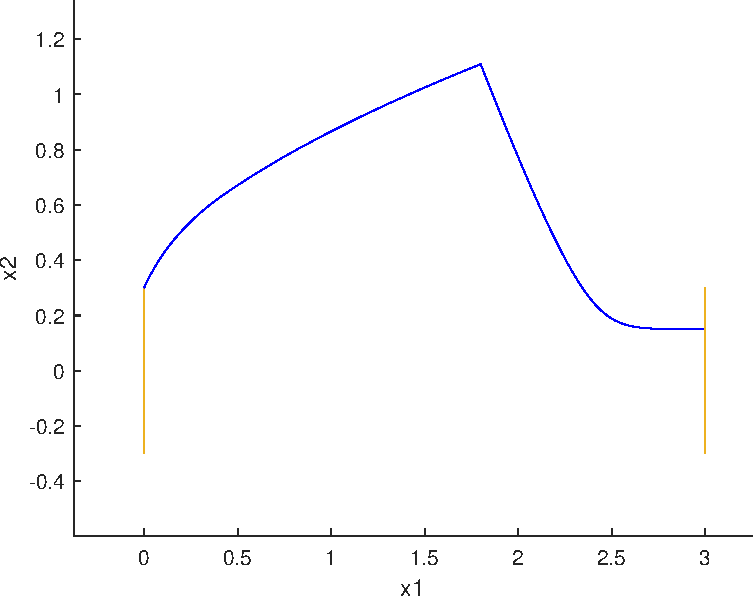
\includegraphics[width=7cm]{Phase_space_1.pdf} }}
    \qquad
    \subfloat[\centering Графики компонент оптимального управления \( u(t) \).]{{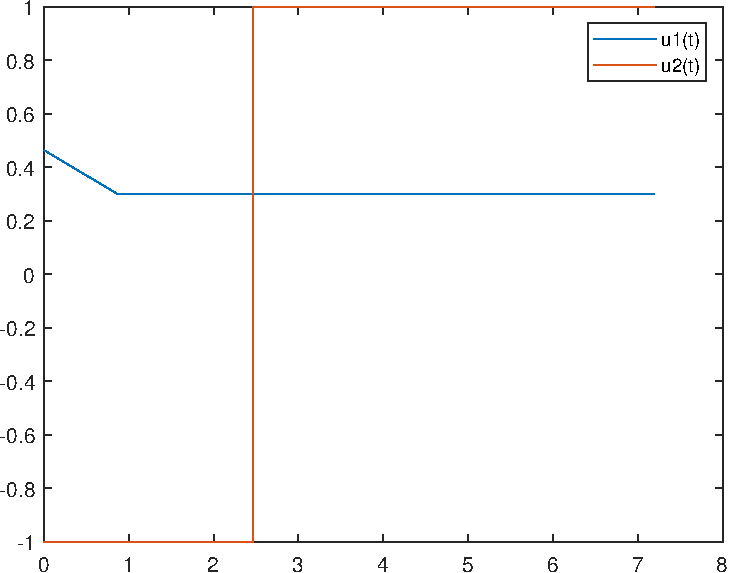
\includegraphics[width=7cm]{u(t)_1.pdf} }}
    \\
    \subfloat[\centering Графики компонент оптимальной траектории \( x(t) \).]{{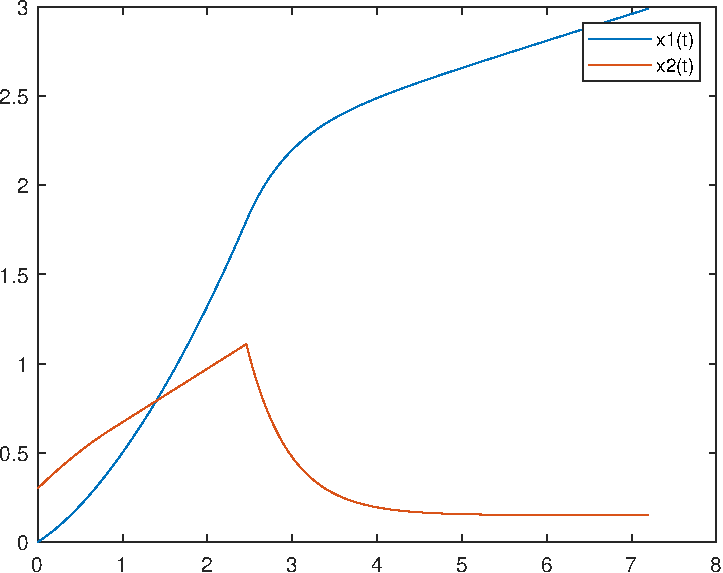
\includegraphics[width=7cm]{x(t)_1.pdf} }}
    \qquad
    \subfloat[\centering Графики компонент сопряженной переменной \( \psi(t) \).]{{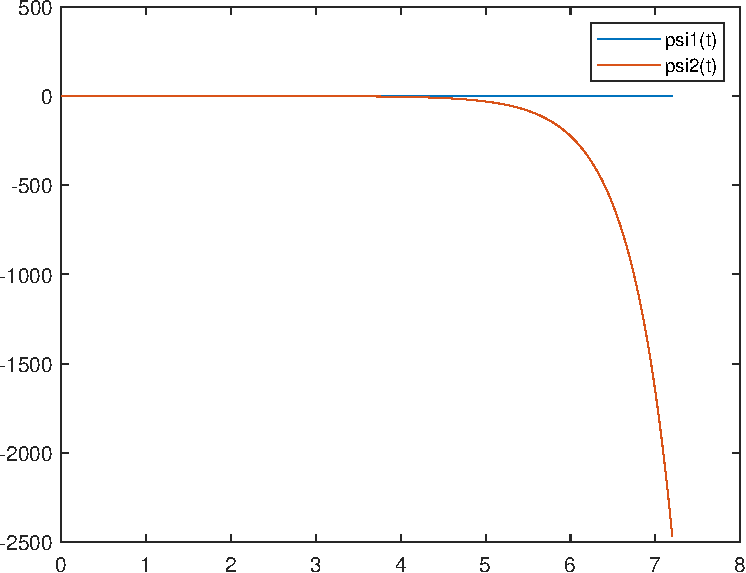
\includegraphics[width=7cm]{psi(t)_1.pdf} }}
\end{figure}
\newpage

\anonsubsection{Пример 2}
\[ \mathcal{P} = \mathcal{P}_1, T = 19.5 , \varepsilon = 0.3, u_{min} = 0.3, k = 1, L = 3, \] 
\[ \text{absTol = 1e-7, relTol = 1e-6, iters0 = 50 , iters1 = 60, mist = 0.01} \].

\begin{figure}[h]
    \centering
    \subfloat[\centering Траектории системы в фазовом пространстве.]{{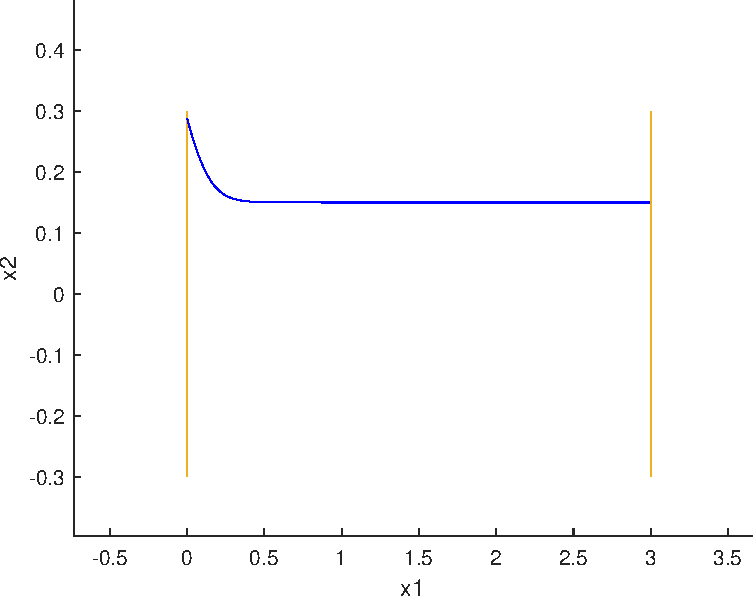
\includegraphics[width=7cm]{Phase_space_2.pdf} }}
    \qquad
    \subfloat[\centering Графики компонент оптимального управления \( u(t) \).]{{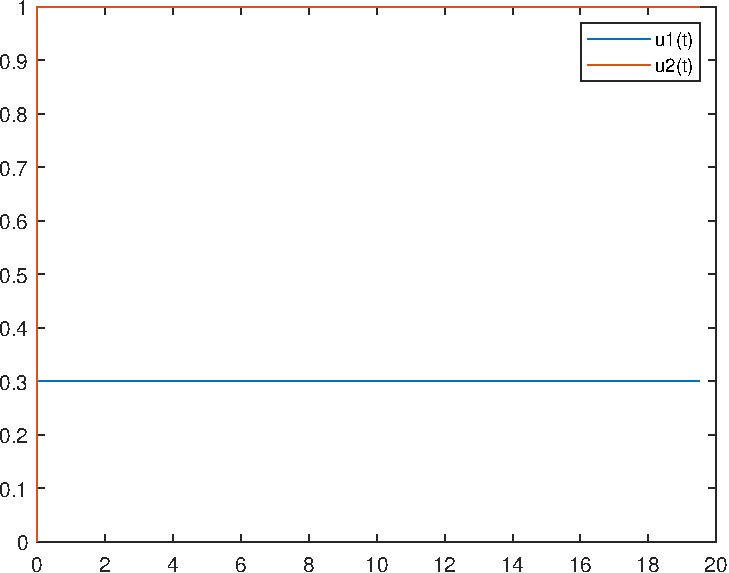
\includegraphics[width=7cm]{u(t)_2.pdf} }}
    \\
    \subfloat[\centering Графики компонент оптимальной траектории \( x(t) \).]{{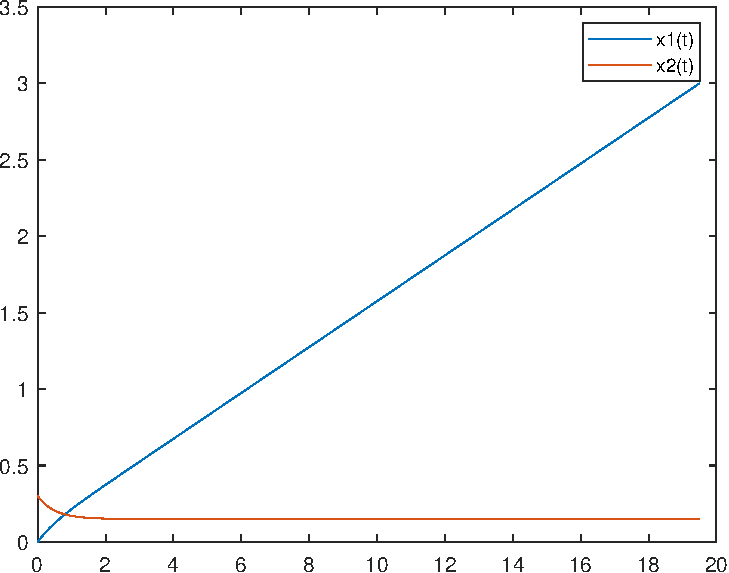
\includegraphics[width=7cm]{x(t)_2.pdf} }}
    \qquad
    \subfloat[\centering Графики компонент сопряженной переменной \( \psi(t) \).]{{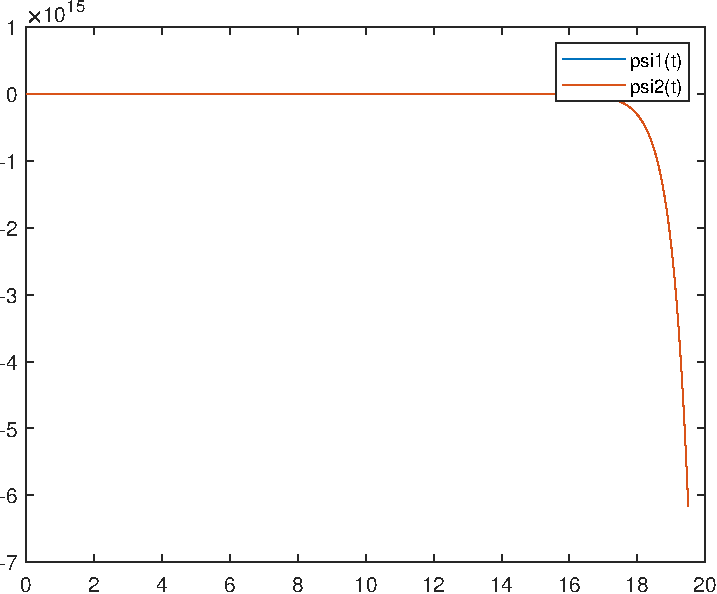
\includegraphics[width=7cm]{psi(t)_2.pdf} }}
\end{figure}
\newpage

\anonsubsection{Пример 3}
\[ \mathcal{P} = \mathcal{P}_1, T = 4.05 , \varepsilon = 0.3, u_{min} = 0.3, k = 0.9, L = 3, \] 
\[ \text{absTol = 1e-7, relTol = 1e-6, iters0 = 30 , iters1 = 50, mist = 0.01} \].

\begin{figure}[h]
    \centering
    \subfloat[\centering Траектории системы в фазовом пространстве.]{{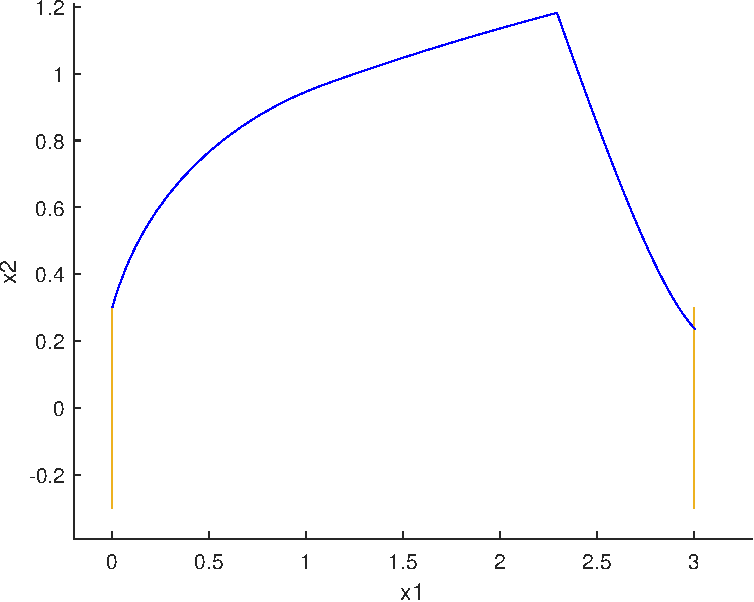
\includegraphics[width=7cm]{Phase_space_3.pdf} }}
    \qquad
    \subfloat[\centering Графики компонент оптимального управления \( u(t) \).]{{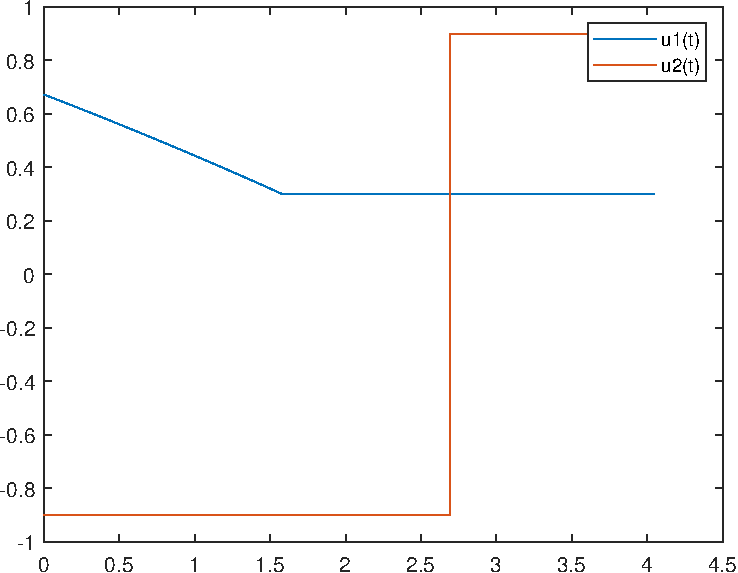
\includegraphics[width=7cm]{u(t)_3.pdf} }}
    \\
    \subfloat[\centering Графики компонент оптимальной траектории \( x(t) \).]{{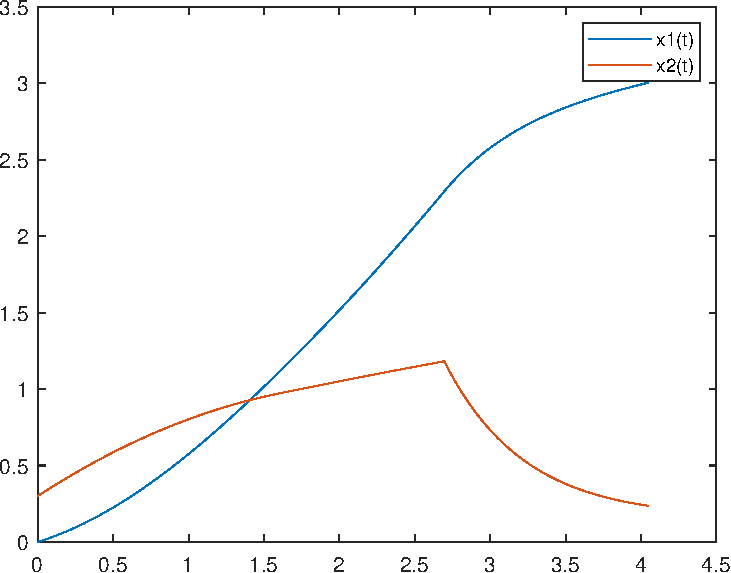
\includegraphics[width=7cm]{x(t)_3.pdf} }}
    \qquad
    \subfloat[\centering Графики компонент сопряженной переменной \( \psi(t) \).]{{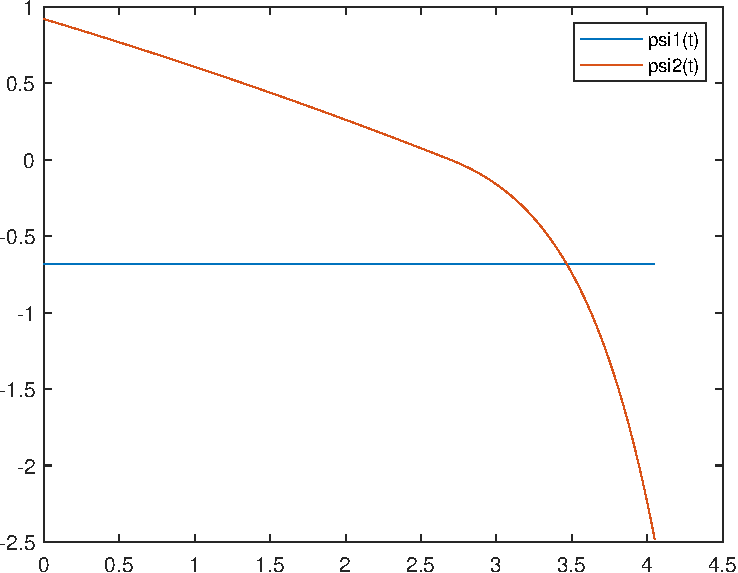
\includegraphics[width=7cm]{psi(t)_3.pdf} }}
\end{figure}
\newpage

\begin{thebibliography}{0}
\addcontentsline{toc}{section}{Список литературы}
\bibitem{1}
Ю.\,Н. Киселев, С.\,Н. Аввакумов, М.\,В. Орлов \emph{Оптимальное управление. Линейная теория и приложения:Учебное пособие} М.:МАКС Пресс, 2007
\bibitem{2}
Л.\,С. Понтрягин, В.\,Г. Болтянский , Р.\,В. Гамкрелидзе , Е.\,Ф. Мищенко \emph{Математическая теория оптимальных процессов} М.: Наука, 1983
\end{thebibliography}
\end{document}